\section{Matplotlib} % (fold)
\label{sec:section_name}

\begin{frame}
\frametitle{What is Matplotlib?}


\begin{itemize}
    \item Plotting library for Python
    \item Works well with Numpy
    \item Syntax similar to Matlab
\end{itemize}

\end{frame}

\begin{frame}
\frametitle{Scatter Plot}
\lstset{basicstyle=\scriptsize}
\codeblock{code/mpl_line_plot.py}
\begin{figure}[h]
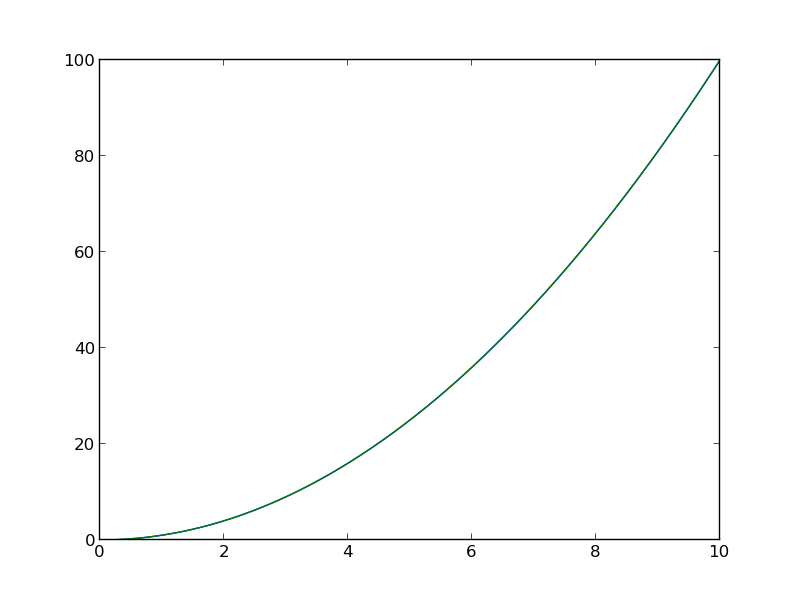
\includegraphics[width=.6\textwidth]{img/line_plot.png}
\end{figure}
\end{frame}

\begin{frame}
\frametitle{Seaborn makes plot pretty}
\lstset{basicstyle=\scriptsize}
\codeblock{code/mpl_line_plot_sns.py}
\begin{figure}[h]
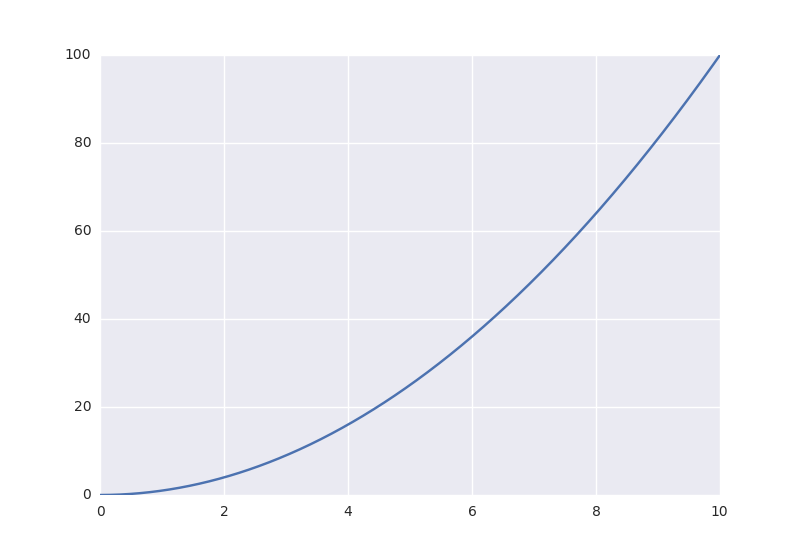
\includegraphics[width=.6\textwidth]{img/lineplot_sns.png}
\end{figure}
\end{frame}


\begin{frame}
Adding titles and labels
\frametitle{Scatter Plot}
\codeblock{code/mpl_line_plot_plus.py}
\end{frame}

\begin{frame}
\frametitle{Scatter Plot}
\begin{figure}[h]
\centering
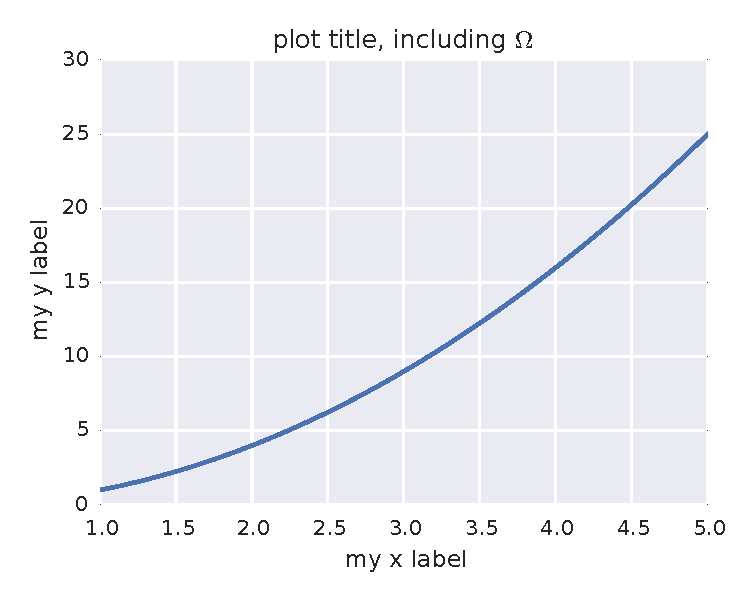
\includegraphics[width=.9\textwidth]{img/line_plot_plus.pdf}
\end{figure}
\end{frame}

\begin{frame}
\frametitle{Scatter Plot}
Adding multiple lines and a legend
\lstset{basicstyle=\small}
\codeblock{code/mpl_line_plot_plus2.py}
\end{frame}

\begin{frame}
\frametitle{Scatter Plot}
\begin{figure}[h]
\centering
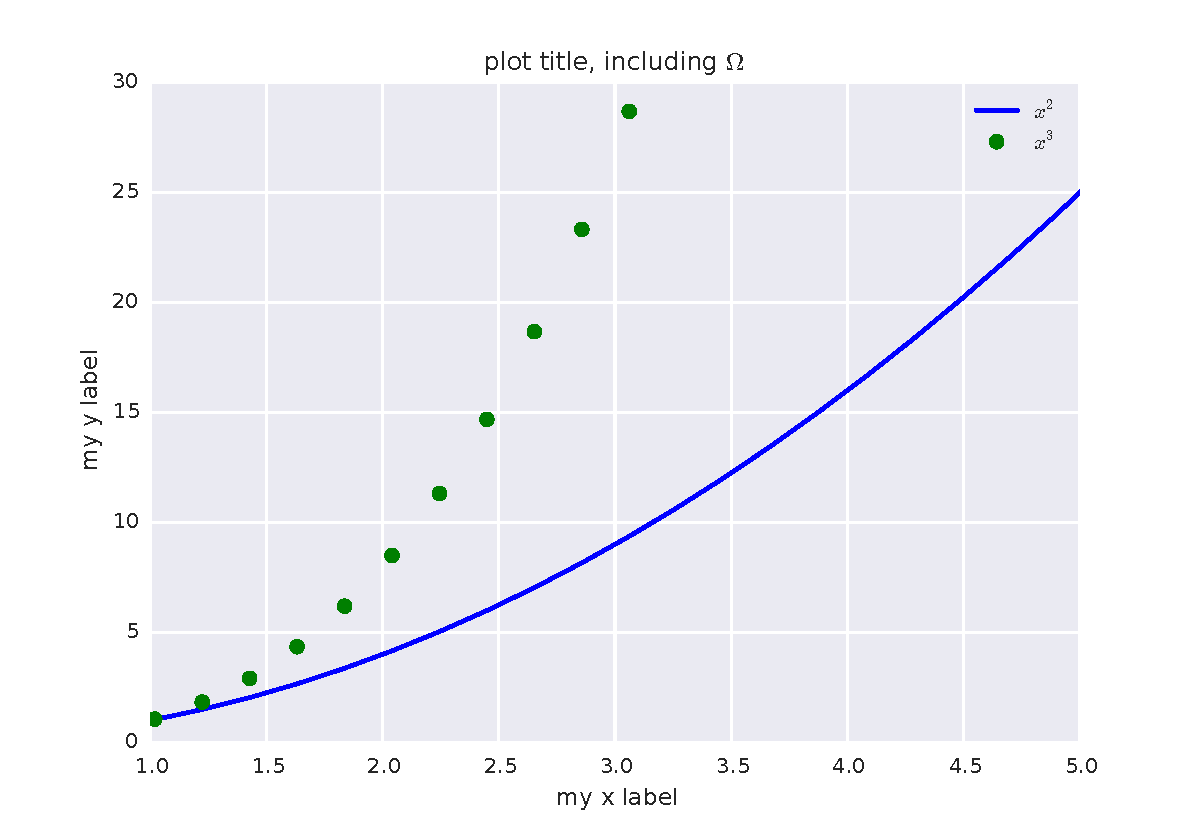
\includegraphics[width=.9\textwidth]{img/line_plot_plus2.pdf}
\end{figure}
\end{frame}


\begin{frame}
\frametitle{Histogram}
\lstset{basicstyle=\small}
\codeblock{code/mpl_histogram.py}
\end{frame}

\begin{frame}
\frametitle{Histogram}
\begin{figure}[h]
\centering
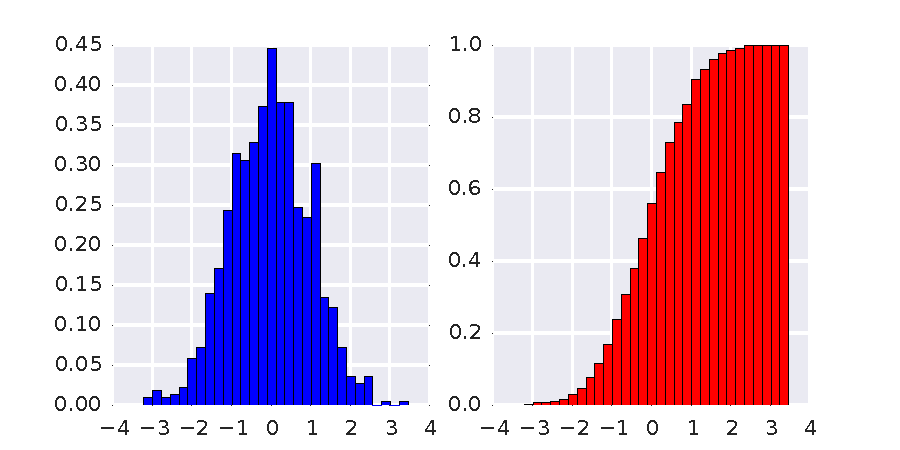
\includegraphics[width=.9\textwidth]{img/histogram.pdf}
\end{figure}
\end{frame}


\begin{frame}
\frametitle{Box Plot}
\codeblock{code/mpl_boxplot.py}
\end{frame}

\begin{frame}
\frametitle{Box Plot}
\begin{figure}[h]
\centering
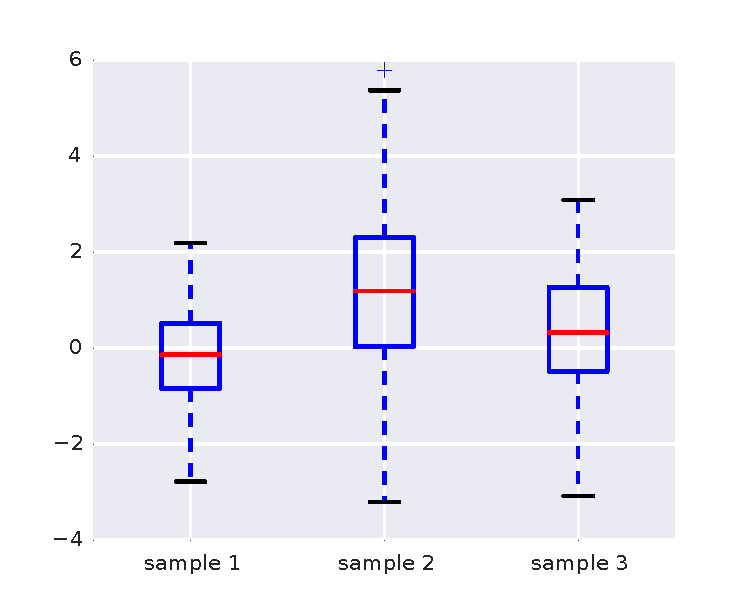
\includegraphics[width=.9\textwidth]{img/boxplot.pdf}
\end{figure}
\end{frame}


\begin{frame}
\frametitle{Image Plot}
\codeblock{code/mpl_imageplot.py}
\end{frame}

\begin{frame}
\frametitle{Image Plot}
\begin{figure}[h]
\centering
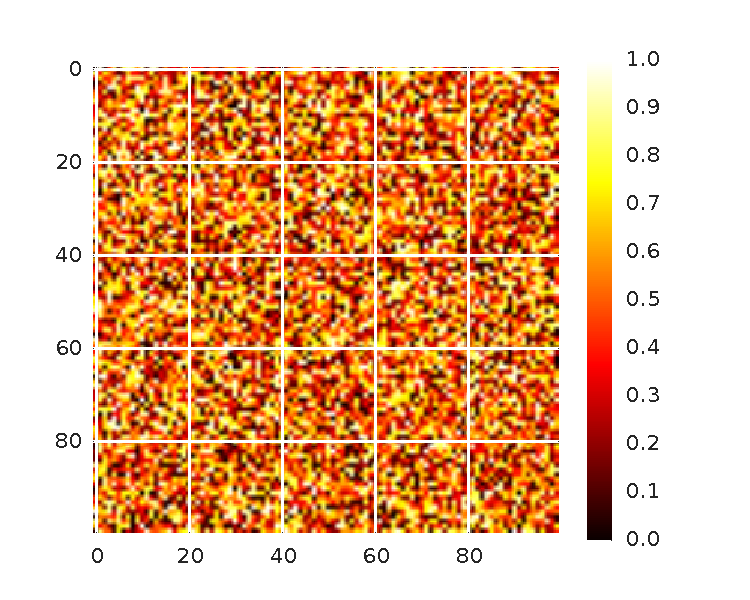
\includegraphics[width=.9\textwidth]{img/imageplot.pdf}
\end{figure}
\end{frame}


\begin{frame}
\frametitle{Wire Plot}
matplotlib toolkits extend funtionality for other kinds of visualization
\codeblock{code/mpl_wire.py}
\end{frame}

\begin{frame}
\frametitle{Wire Plot}
\begin{figure}[h]
\centering
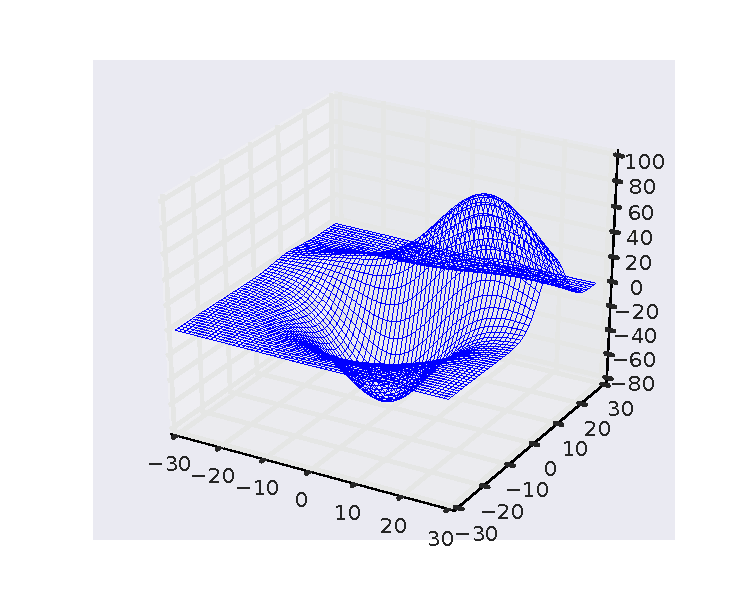
\includegraphics[width=.9\textwidth]{img/wire.pdf}
\end{figure}
\end{frame}

\begin{frame}\frametitle{Possibilities}

A lot is possible, but not always easy to figure out how...

\begin{figure}[h]
\centering
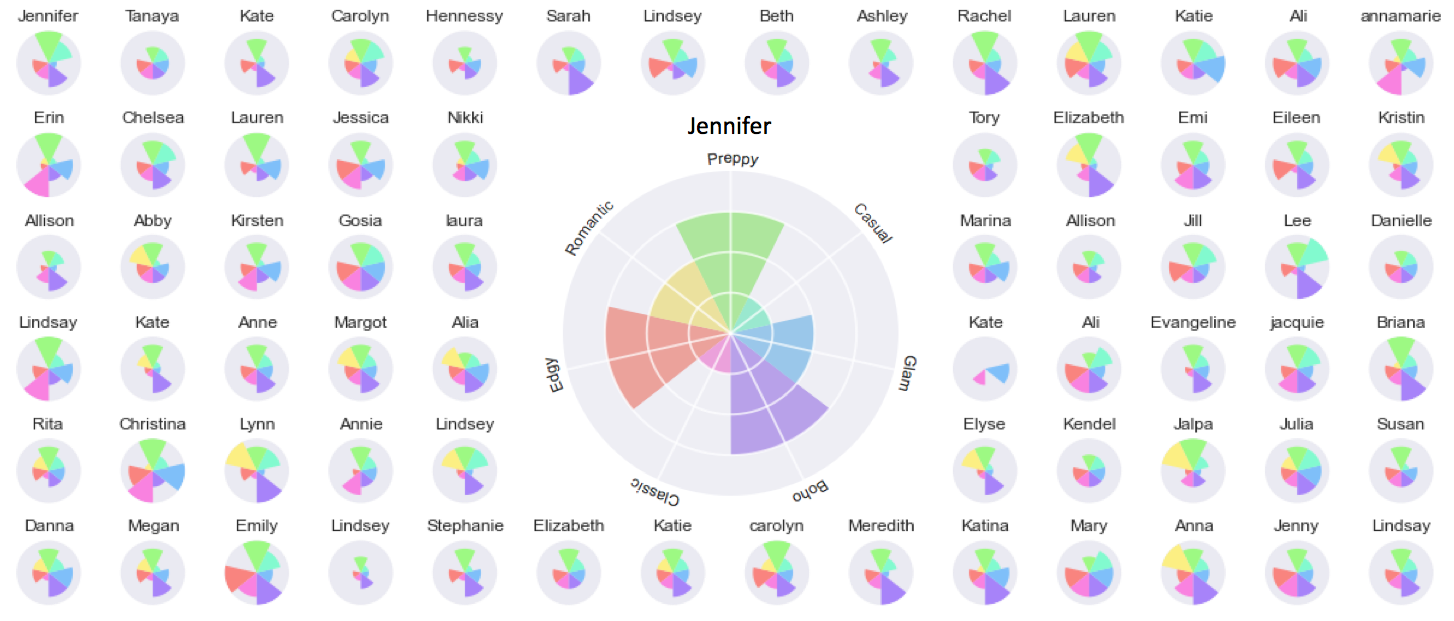
\includegraphics[width=.9\textwidth]{img/sf_vectors.png}
\end{figure}

\end{frame}

% section section_name (end)
